% !!! 本文件由 work/tools/gen_index.py 生成，请勿手改 !!!
% 想调整章序 / 部分划分：改 gen_index.py 顶部的 PARTS / LOOSE / BACK_PAGES。

\begin{center}
\thispagestyle{empty}
\begin{tikzpicture}[remember picture, overlay, inner sep=0pt]
\node at (current page.center)
{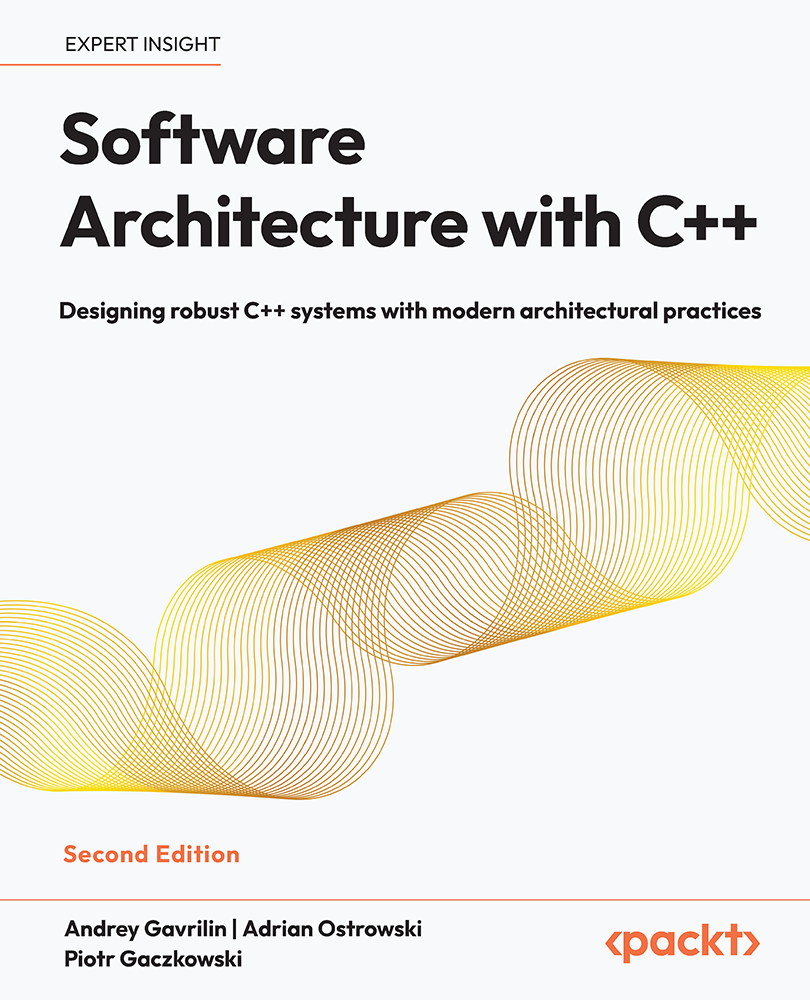
\includegraphics[width=\paperwidth,height=\paperheight,keepaspectratio]{images/cover.png}};
\end{tikzpicture}
\end{center}

\myFrontNoToc{content/front/00-title}

\newpage
\thispagestyle{empty}
\tableofcontents
\newpage

\myFront{贡献者}{content/front/01-contributors}

\myFront{前言}{content/front/02-preface}

\myPart{1}{软件架构的概念与组件}{content/part/01}

\myChapter{1}{软件架构的重要性\\与优秀的设计原则}{content/main/01}

\myChapter{2}{架构风格}{content/main/02}

\myChapter{3}{功能性需求与非功能性需求}{content/main/03}

\myPart{2}{C++ 软件的设计与开发}{content/part/02}

\myChapter{4}{架构与系统设计模式}{content/main/04}

\myChapter{5}{利用 C++ 语言特性}{content/main/05}

\myChapter{6}{设计模式与 C++ 惯用法}{content/main/06}

\myChapter{7}{构建与打包}{content/main/07}

\myChapter{8}{包管理}{content/main/08}

\myChapter{9}{C++ 代码复用的未来：使用模块}{content/main/09}

\myPart{3}{架构质量属性}{content/part/03}

\myChapter{10}{编写可测试的代码}{content/main/10}

\myChapter{11}{持续集成与持续部署}{content/main/11}

\myChapter{12}{代码与部署中的安全性}{content/main/12}

\myChapter{13}{性能}{content/main/13}

\myPart{4}{云原生设计原则}{content/part/04}

\myChapter{14}{分布式系统的架构}{content/main/14}

\myChapter{15}{服务间通信}{content/main/15}

\myChapter{16}{容器}{content/main/16}

\myChapter{17}{可观测性}{content/main/17}

\myChapter{18}{云原生设计}{content/main/18}

\myChapter{19}{解锁本书的专属权益}{content/main/19}

\myFront{测评题解答}{content/back/assessments}

\myFront{订阅通讯}{content/back/newsletter}

\myFront{其他可能感兴趣的书}{content/back/other-books}

\myFront{索引}{content/front/index}
